
\subsection{L'évaluation par la construction, une mise en pratique de la validation}
\label{ssec:evaluation_construction}

% Permanence des questions évoqués pour la construction d'un modèle de simulation, plus complexification de la validation liés à la pluriformalisation.

En montrant que la validation est dépendante au contexte, Hermann a permis de lever un certain nombre de questions remarquable par leur actualité dans le cadre de nos propre problématique de construction.  %La mise en avant d'une possibilité de validation dépendante à l'objectif nous oblige inévitablement à prendre en compte l'activité de construction comme activité validante.

\subsubsection{Des modalités de validation dépendante au contexte, l'apport d'Hermann à une première formalisation du problème}

\paragraph{Une vision de la validation différente chez les pionniers du mouvement S\&G}

Charles F. Hermann opère dans la branche des simulations appelés à l'époque par Shubik les \textit{Man-Machine Games} \autocite{Shubik1972}. Une catégorie de simulation qui intègre dans son exécution un couplage entre un ou plusieurs systèmes numériques et des humains, qui peuvent être amené à interagir entre eux, ou avec les machines. Ce type de simulation de structure hétérogène est intéressante dans le sens ou elle permet d'intégrer l'arbitraire humain dans une chaîne d'interaction complexe qui n'aurait pas pu être établi autrement, du fait de l'impossibilité de programmer des interactions et des réactions humaines face à des situations précises. Même si ce type de techniques est motivé par une multitude d'usages, ce n'est pas par hasard si elle se développe particulièrement au cours de la guerre froide aux états-unis, toujours sous la direction d'institution militaires. Ce genre de techniques permettant par exemple de simuler et de reproduire des guerres au travers d'inter-relations diplomatiques et/ou économiques \autocite{Hermann1967b}, avec la possibilité de mesurer via des indicateurs adaptés l'importance et l'impact de différents scénarii sur le couple humain/machine.

Ce type de simulation est particulièrement représenté dans des publications qui traitent de la simulation au sens large, comme par exemple le journal \textit{Simulation and Gaming} ou \textit{S\&G} \autocite{Crookall2011}, dont l'activité remonte au début des années 1970. On retrouve parmi les auteurs ayant participé au développement de la discipline des personnalités importantes comme Guetzkow, Shubik, Coleman, etc. \autocite{Crookall2012}. Aujourd'hui, le terme à évolué vers ce que l'on pourrait probablement appeler des jeux sérieux, l'utilisation de l'ordinateur n'étant plus forcément un élément obligatoire dans ce type de simulation. Du côté des objectifs qui sont aujourd'hui susceptibles de motiver l'utilisation de ces techniques, \textcite{Shubik2009} définit une taxonomie en 6 objectifs : \textit{teaching, experimentation, entertainment, therapy and diagnosis, operations, training }

Cette présence d'une dimension humaine dans les simulations introduit une complexité qui touche forcément à plusieurs objets d'études des sciences humaines (psychologie, sociologie, etc.), et il n'est donc pas étonnant que l'on retrouve ce type de publication dès l'apparition des premiers ouvrages inter-disciplinaires sur la simulation, quand elle ne les pilote pas; Harold Guetzkow par exemple est un des personnages importants qui gravitent autour de Herbert Simon au GSIA (Graduate School of Industrial Administration) de Carnegie Tech dans les années 1950-56 \autocite{Guetzkow2004}, et qui a beaucoup oeuvré pour le développement de la simulation dans ces sciences politiques et psychologiques (\textit{Inter-Nation simulation laboratory}) \autocite{Janda2011, Druckman2010}. Celui ci s'inscrit exactement dans la même branche que Hermann, et apparaît deux fois comme premier éditeur dans des recueils de textes pluri-disciplinaires traitant de la simulation au sens large, preuve aussi de son implication dans le développement et la diffusion de ces techniques au delà de sa propre discipline \autocite{Guetzkow1962, Guetzkow1972}

\paragraph{L'apport du contexte dans l'évolution du sens attaché à l'activité de simulation}

Ce qui est intéressant dans ce type de simulations, c'est qu'elles forcent à penser la validation des modèles sous un angle qui doit nécessairement tenir compte de la variabilité inhérente aux comportements humains, par essence difficilement évaluables et réplicables. C'est de cette contrainte, et parce que \textcite{Hermann1967} s'intéresse au modèle de simulation pour d'autres objectifs que la prédiction (\textit{teaching, training, theory-building}), que celui-ci développe à mon sens une vision de la validation beaucoup plus réaliste pour les sciences sociales que celle proposée à la même période par Naylor.

\foreignquote{english}{First, the validity of an operating system is affected by the purpose or use for which the game or simulation is constructed [...]}\autocite[217]{Hermann1967}

% Plus d'information à ajouter, soit sur la dite boucle (sachant que le conceptual correspond quand meme pas mal à ce que lon fait, voir Sargent2010), Si la boucle définit par les tenants de la \textit{V\&V} n'est pas inintéressante, et de façon générale résume bien le cycle de vie qui correspond à la construction d'une simulation, de nombreuses questions reste en suspens sur le choix et la mise en œuvre des techniques telles qu'elles sont décrites. La construction et la mise en oeuvre des critères en fait partie. Les objectifs sont cités dans la définitions mais on ne rentre pourtant pas dans le détail de la relation entre ces objectifs et la construction du modèle, qui est laissé à l'expertise de l'utilisateur, en cela Hermann ne propose pas mieux dans sa description d'une boucle modélisatrice que les dernières avancées portés par Sargent2010, toutefois sa réflexion est par son orientation, et par sa précocité de réflexion son intéressante il me semble à citer. les moyens technique de la mise en oeuvre par exemple ? 

%Dans l'explication sociologique, la réalité structurelle n'est pas forcément d'intérét pour la construction du modèle. (bulle)

%Cette observation amène Hermann à considérer que la validation des composantes de la structure mérite une attention tout aussi importante que la seule comparaison avec des données de sorties, notamment dans un cadre explicatif.  curl -k -o ~/backups/pinboard-backups/pinboard-$(date +\%y\%m\%d).json 'https://api.pinboard.in/v1/posts/all?&auth_token=username:APItokenhere&format=json'

En s'appuyant sur ce premier argument évoquant l'existence d'une dépendance liant processus de validation et objectif poursuivis par le modélisateur, Hermann semble \textit{de facto} mettre en défaut une définition de la simulation ayant comme première et unique vocation à représenter au mieux le système observé.

\Anotecontent{hermann_modalite}{\foreignquote{english}{The first comment is that the validation of an operating model cannot be separated from the purpose for which it is designed and used. [...] The second observation somewhat mediates the first. For the most part the various purposes for conducting games and simulations do not negate the need for criteria we can use to estimate the degree of fidelity with which one system (the operating model) reproduces aspects of another (the reference system). Given some purposes for using games and simulations (such as exploring nonexistent universes), finding appropriate criteria in the referent system is quite difficult. With other objectives, the value of the operating model may remain even if the fit between the model and various criteria representing the observable universe is poor (as in theory building).} \autocite[219]{Hermann1967}}

La discussion qui suit sur l'existence de multiples objectifs de modélisation permet à Hermann de révéler la diversité et l'attachement de la validation à un contexte, et de noter d'une part comment la variation de ce dernier affecte les modalités de cette comparaison entre système simulé et système observé, et d'autre part comment cela affecte la perception du résultat engendré par cette comparaison.\Anote{hermann_modalite}

Indirectement, on observe donc ici le tranfert d'une définition de la simulation comme simple \enquote{type de modèle} vers la définition plus générale d'une simulation \enquote{ caractérisée non pas tant par l’unité d’une fonction cognitive qu’elle assurerait toujours sous une forme ou sous une autre que par son fonctionnement interne, fonctionnement qui, bien sûr, mais seulement secondairement, se trouve avoir aussi des conséquences sur sa ou ses fonctions cognitives. Une simulation nous paraît ainsi devoir être prioritairement caractérisée par ce qu’elle est – ou fait – de manière interne plutôt que par ce qu’elle fait au sens d’une fonction cognitive quelconque qu’elle assurerait toujours et qu’on en attendrait prioritairement de l’extérieur : à ce titre, nous proposons de dire qu’\textit{elle est avant tout un traitement spécifique sur des symboles et qui prend toujours la forme d'au moins deux phases distinctes. 1) une phase opératoire [...] 2) une phase d'observation [...]}} \autocite[33-34]{Varenne2013}

\Anotecontent{naylor_etonnement}{On pourra peut être être étonné de retrouver la démarche de Naylor dans les approches subjectives sachant la description qu'on en a fait au préalable. Mais il y a bien une part de subjectivité dans cette démarche, l'application de chacune des étapes de la multi-stage validation faisant quand même appel à une forme d'expertise pour constituer le jeu des hypothèses que l'on estime valable en vue du test final de comparaison aux données.}

L'acceptation d'un gradient de valeur pour juger de la validation rompt avec la méthode \enquote{binaire} proposé par Naylor, la validation d'un modèle passant à présent par l'acceptation subjective d'un seuil de représentativité relatif à l'objectif poursuivis. Avec pour conséquence notable qu'une \foreignquote{english}{[...] simulation or game relatively valid for one objective may be not be equally valid for another.}

Si la notion de seuil n'est pas explicitement abordé par Hermann, c'est pourtant sous cette aceptation que la \textit{V\&V} actuelle va reprendre ce concept. Avec la position suivante, celui de se fixer un seuil de représentativité général à atteindre \textit{a priori}, une contrainte peu réaliste dans le cadre des sciences humaines, ou quantifier par avance un tel seuil n'aurait pas de sens. 

\foreignquote{english}{\textbf{Principle 2: The outcome of simulation model VV\&T should not be considered as a binary variable where the model is absolutely correct or absolutely incorrect } [...] The outcome of model VV\&T should be considered as a degree of credibility on a scale from 0 to 100, where 0 represents absolutely incorrect and 100 represents absolutely correct. 

\textbf{Principle 3: A simulation model is built with respect to the study objectives and its credibility is judged with respect to those objectives } [...]The study objectives dictate how representative the model should be. Sometimes, 60\% representation accuracy may be sufficient; sometimes, 95\% accuracy may be required depending on the importance of the decisions that will be made based on the simulation results. Therefore, model credibility must be judged with respect to the study objectives.}\autocite[15-16]{Balci1998}

La position de \textcite[166]{Sargent2010}, tout en étant relativement similaire, propose une vision plus fine et plus réaliste ou le seuil de précision attendu est attaché aux variables de sorties. Un point important sur lequel nous reviendrons plus longuement dans la suite de cette partie. \hl{ref vers la bonne partie}

\foreignquote{english}{A model should be developed for a specific purpose (or application) and its validity determined with respect to that purpose.[...] A model is considered valid for a set of experimental conditions if the model’s accuracy is within its acceptable range, which is the amount of accuracy required for the model’s intended purpose. This usually requires that the model’s output variables of interest (i.e., the model variables used in answering the questions that the model is being developed to answer) be identified and that their required amount of accuracy be specified. The amount of accuracy required should be specified prior to starting the development of the model or very early in the model development process.}\autocite[166]{Sargent2010}

Ces deux citations permettent de montrer au passage comment la vision de la validation défendu par Hermann a été intégrés dans une forme très approchante par des acteurs de la \textit{V\&V} comme Balci ou Sargent, dont on a vu précédemment les définitions dans la section \ref{ssec:def_generique_validation}. Ces deux derniers sont en réalité les acteurs majeurs d'une synthèse (voir la figure \ref{fig:S_syntheseBalci}) opéré dans les années 1980-1990 \autocite{Nance2002}, dont on peut dire qu'elle est marqué par un retour à une certaine forme de neutralité (voir par exemple le rejet des aspects philosophiques décrits décrits dans la section \ref{ssec:def_generique_ validation}  qui se double d'un jargon technique spécifique à l'établissement d'un processus qualité exploitable pour l'ingénierie) . Des adaptation qui permettent probablement de mieux accepter en son sein des typologies de techniques aussi différentes que celle de Naylor\Anote{naylor_etonnement} ou Hermann. Régulièrement révisées, \textcite{Balci1998} fait ainsi état dans sa dernière taxonomie d'un catalogue de 75 techniques différentes dans lequel peuvent piocher les modélisateurs en fonction de leur besoins. 

\begin{figure}[h]
\begin{sidecaption}[fortoc]{ On remarquera la forte présence des techniques présentés par Hermann dans la synthèse proposé par Balci en 1986 \autocite{Balci1986}}[fig:S_syntheseBalci]
  \centering
 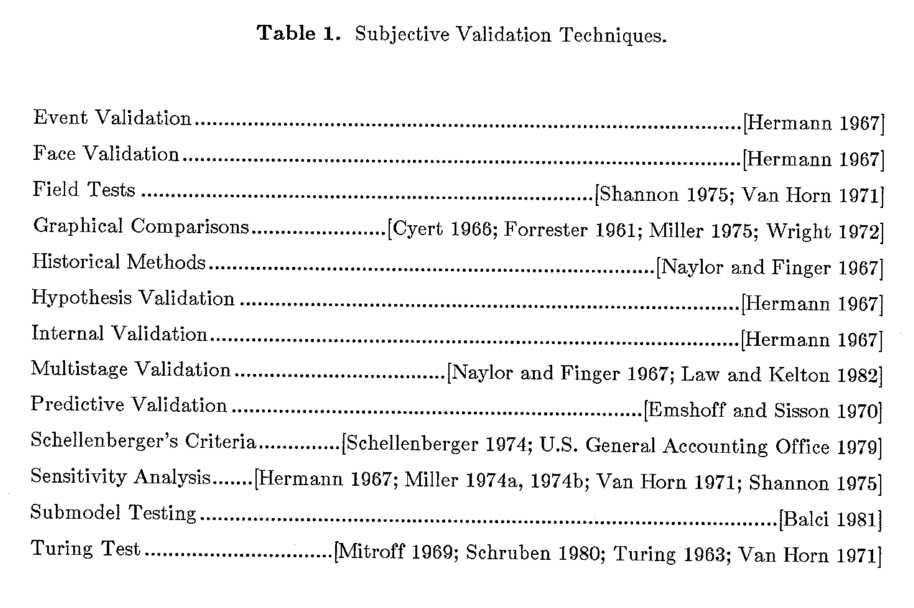
\includegraphics[width=.9\linewidth]{subjective_balci.png}
  \end{sidecaption}
\end{figure}

Les modalités de la validation étant maintenant défini par rapport au contexte, la possibilité d'un critère unique pour juger de la validation de façon universelle paraît improbable. Afin de montrer qu'il ne s'agit pas seulement d'une question de disponibilités des données, et pour amener par la suite sa proposition de méthode multi critères, Hermann s'attaque donc en premier lieu à réduire la portée des confirmations apportés sur un système observés par l'emploi de la seule technique de validation basé sur la comparaison de données en sortie des modèles de simulation.

\paragraph{Les limites d'une validation basé sur le critère de la comparaison historique}

Pour montrer qu'il existe des limitations dans la confiance que l'on peut mettre dans la validation lorsqu'il s'agit de comparer des données historiques (dans le cas des simulations de reproduction de guerre, on parle ici plutôt de reproduire des séries d'événements historiques) -cela même si elles sont idéalement toute rendues disponible- aux données en sorties de simulation, \textcite{Hermann1967b} s'appuient sur les travaux de \textcite{Pool1965}.

\foreignquote{english}{This correspondence does not demonstrate that the simulation correctly represents the structure and processes that were operative in the historical occurence. We are speculating on the similarity between the historical and simulated inputs on the basis of the similarity of their outputs. Different relationships among various combination of properties in the simulation conceivably could produce outcomes like those in the historical situation.

A simulation of the 1960 national Presidential election predicted the percentage of the vote for each candidate - the outcome - with considerable success. The designers of that simulation observe, however, that \enquote{it may legitimaly be asked what in the equations accounted for this success, and whether there were parts of the equations in the simulation that contributed nothing or even did harm} Further analysis of the equations in the simulation revealed that the outcome was predicted despite the fact that at least one equation misrepresented aspects of voter turnout. Part of the structure was incorrect, but the simulated result still matched the actual outcome. Despite this difficulty, our confidence that the simulation has captured some aspects of the voting process is greater than it would have been if the simulation had failed to replicate the campaign outcome. Confidence in the simulation would increase further as the operating model demonstrated ability to produce outcomes that corresponded with various elections. In sum, the similarity between simulation and historical events can provide at best only indirect and partial evidence for the correctness of the simulated structures and processes that produced the outcome.}

Ce que nous dit Hermann ici, à la différence de Naylor, c'est que même dans le cas idéal ou toutes les données serait présente, ce mode classique de validation ne peut pas être suffisant, cela quelque soit l'objectif poursuivis par le modélisateur. Un constat que nous avions déjà acquis à la lecture des déboires des géographes avec les préceptes de validation néo-positivistes, associant dans une démarche de modélisation instrumentaliste prédiction et explication (section \ref{sssec:realite_neopositiviste}).

Ce constat reste encore valide aujourd'hui et cela indépendamment de la technique utilisée. Ainsi, \textcite[106]{Amblard2006} nous rappelle que dans le cadre des modèles agents, où le modélisateur cherche à évaluer la portée explicative de ses hypothèses, \enquote{[...] la recherche de similitudes avec les données, si elle peut être utile, ne peut absolument pas être un critère unique et définitif de validation}

\hl{Trouver une question ? ou faut il directement poser ici les hypothèses de la validation multi critères, tout en la discutant par la suite ? }

Pour comprendre en quoi la proposition d'Hermann est encore aujourd'hui une base pertinente et originale pour développer une réflexion sur la validation dans les sciences humaines, il est nécessaire d'évoquer et de discuter dans la suite de cette argumentaire les problématiques qui justifient selon lui d'adopter une validation multi-critère pour la validation : \foreignquote{english}{We have arrived at the position, then, that multiple validity criteria are needed because of the error of measurement and because of the recognition that criteria can be only assertions about \enquote{reality}}. 

Une reflexion qui se niche dans l'observation des modalités de construction des deux systèmes modélisé et observé, la question de la \enquote{représentativité} se présentant comme le résultat d'une confrontation entre ces deux objets, et cela au regard de l'objectif poursuivi par le modélisateur.

\subsubsection{Le problème de la validation ramené à une confrontation des représentations entre système modélisé et système observé}
\label{ssec:confrontation_sysmodelise_sysobserve}

\foreignquote{english}{A simulation or game is the partial representation of some independent system. Usually we are interested in simulation as a means for increasing our understanding of the system it is intended to copy. Therefore, the representativeness of a simulation or game becomes extremely important in assessing its value. The process of determining how well one system replicates properties of some other system is called validation.[...] In the present analysis however, validation will be defined more broadly as any comparison between the representation of a system and specified criteria} \autocite[216]{Hermann1967}

\hl{repetition ?}
La question de la représentativité d'une simulation est un sujet délicat à traiter car sa valeur se dessine à l'intersection d'au moins deux activités, la construction d'un modèle opérationel et la construction d'une grille d'évaluation, deux activités dont on s'apercoit par la suite qu'elles sont en réalité étroitement liées. 

\subsubsection{La construction d'un modèle de simulation opérationel : Quelles hypothèses pour quelle représentativité ?}
\label{sssec:hypothese_representativite}

La V\&V a toujours mis en avant le fait que la modélisation soit un processus incrémental tout à fait nécessaire pour obtenir un modèle de simulation satisfaisant, que cela soit dans les analyses de Naylor, ou d'Hermann. Ce dernier se réfère en 1967 au principe de parcimonie, une méthode qui implique une abstraction, une simplification du système à représenter, et qui pour lui met logiquement et automatiquement en péril la représentativité. \Anote{Herman_parcimonie} 

\hl{INTEGRER ICI LA REFLEXION HERBERT SIMON sur Hypothèse simplifié, mais également la réflexion d'arnaud et cie sur l'activité de construction => PAS SUR EN FAIT}

Une parcimonie hérité du principe d'Ockham dont on sait qu'elle n'est en aucun cas un synonyme de simplicité dans sa mise en oeuvre, celle-ci nécessitant au contraire un effort intellectuel important pour déterminer quelles sont les hypothèses réellement représentatives du problèmes à analyser. Sur le plan de complexité, Poincarré ou le prix nobel d'économie Herbert Simon à fait état plusieurs fois des capacités d'expression du complexe rendu possible par l'usage de la simulation .\autocite{Banos2013a}

Seulement, et compte tenu de ce qui a été dit auparavant sur l'importance de l'objectif dans la perception de cette \enquote{représentativité}, Hermann est aussi d'accord pour dire que cette dernière ne fait pas systématiquement la valeur du modèle - tant soit peu qu'on arrive à fixer une valeur -, comme dans le cas de l'explication, ou elle n'intervient que partiellement, tout en restant selon lui nécessaire (voir l'objectif \textit{hypothesis and theory construction}).

Sur ce point Hermann et par la suite les tenants de la V\&V ne nous en diront pas beaucoup plus, en partie du fait de la spécificité de l'activité de modélisation en science humaine et sociale, et en géographie, sur lequel nous allons nous pencher dans la suite de cette argumentation.

\textit{Que faut il entendre ici par partiellement ? Pourquoi doit on conserver une accroche avec le réel ? Quels sont les leviers permettant au géographe de compenser cette perte de représentativité par un gain en compréhension sur le système à étudier ? }

Il semble exister dans la volonté de construire un modèle explicatif deux attracteur possible et apparemment opposé, avec d'une part la volonté de se rattacher à une forme de réalisme au travers de l'injection d'une part maitrisé de réalité tout au long du processus de construction \Anote{durand_observation}, et de l'autre une force qui nous pousse à se détacher de cette même empirie en faisant un certain nombre de choix sur la nature et les interactions entre hypothèses constituantes du modèle.

La sociologue et épistémologue \textcite{Bulle2005} a bien formalisé ce dilemme dans la nécessité pour tout modélisateur de positionner son modèle sur un gradient opposant le réalisme des causes des modèles explicatif\Anote{bulle_modele_explicatif}, au réalisme des effets des modèles descriptif. 

Pour mieux comprendre comment se déduit l'explication d'un tel positionnement sur ce gradient, le mieux est encore de commencer par évoquer un de ces extrême, en invoquant par exemple le modèle universellement connu de Schelling. De par sa portée d'application extremement générale et la nature très abstraite de ces paramètres celui-ci constitue en soit un extreme intéressant pour comprendre où se situe encore l'explication lorsque le détachement de la réalité est tel. Sur ce point, les analyses de \textcite{Bulle2005} et \textcite{Phan2008, Phan2010} se réfèrent principalement à l'essai de \textcite{Sugden2002} pour évoquer quel type de relation entre les deux mondes peut on attendre de ce type de modèle épuré. 

Les résultats qui dérivent de la mise en dynamique des règles dans le modèle de Schelling sont d'une telle universalité, d'une telle robustesse qu'il n'est même plus question de confronter ces résultats à une réalité. A cet égard le potentiel explicatif de ce type de modèle s'oppose selon \textcite{Bulle2005} à tout réalisme empirique. \hl{transition?}

De ce point de vue, \enquote{le modèle n'est pas tant une abstraction de la réalité qu’une réalité parallèle [...] bien que le monde du modèle soit plus simple que le monde réel, celui-ci n'est pas une simplification de l'autre. Le modèle est réaliste dans le même sens qu'un roman peut être appelé réaliste [...] les personnages et les lieux sont imaginaires, mais l'auteur doit nous convaincre qu'ils sont crédibles } \autocites[131]{Sugden2002}[10]{Phan2008}

L'effet d'une telle recombinaison d'hypothèses revient à mettre en oeuvre un \enquote{monde crédible} où l'inférence inductive est mobilisé pour identifier des similitudes significatives entre les deux mondes. \autocites{Livet2006, Phan2008}. Tout le travail réside donc dans l'interpretation prudente qui peut être faite entre ces résultats d'un monde factice et d'une réalité.

Un processus commun utilisé dans toute oeuvre de fiction pour piquer la curiosité du spectateur/lecteur, la mise en exergue volontaire de tendance du monde réel dans un monde imaginaire permettant d'entamer une réflexion sur l'existence, la portée, la nature de cette même tendance dans le monde réel. Les villes ou les sociétés mis en avant dans des oeuvres de fiction cinéma ou dans la littérature ne sont jamais que des mondes plus ou moins crédibles (Gotham City, 1984, Matrix, la série Black Mirror, etc. car la liste est longue ...)  pour mettre en avant un discours, ou des tendances du monde réel sur lequel doit porter le questionnement; (http://www.influxpress.com/imaginary-cities/ ,  \href{http://cybergeo.revues.org/1170#tocto1n9?}{cybergeo})

Si le discours scientifique n'a clairement pas cette obligation ludique, il n'en reste pas moins que ce processus de reconstruction crédible est un outil formidable pour questionner les processus à l'oeuvre dans le monde réel \Anote{ruffat_samuel_ville}. Mais cette ambiguité de lecture a déjà mené à de nombreux malentendu, d'une part envers le grand public (Voir forrester, mais également \Anote{deffuant_debat}) qui pourrait prendre des résultat de simulation pour la réalité avec tout les conséquences que cela suppose, mais également parfois entre scientifique provenant de divers horizons. Ainsi après la lecture de la critique par \textcite{Chattoe2011} de l'article de \textcite{Yanoff2009}, il ressort toute la difficulté d'évaluer la méthodologie et le travail réalisé autour d'un modèle au travers d'une seule publication, nottament lorsque la fonction cognitive recherché n'est pas vraiment exprimé, ce qui provoque aussi ce décalage entre attente du lecteur et processus réel de recherche qui sous tend la construction du modèle. \hl{Bof à reformuler}

\textit{Mais doit on se contenter d'aussi peu de certitudes ?? Comment peut on renforcer la confiance dans la capacité explicative des hypothèses ainsi mobilisés ? }

\textcite{Bulle2005} evoque bien l'existence de modèle à cheval entre potentialité explicative et potentialité descriptive. Ainsi \enquote{appliquée aux processus sociaux réels, la simulation peut allier au potentiel descriptif offert par l’imitation d’effets empiriquement observables, le potentiel explicatif que lui confère la mise en œuvre de relations causales effectives. }

\hl{+ détail ici sur ce que cela veut vraiment dire ? }

La réintroduction maitrisé de l'empirie dans les modèle de simulation autorise la mise en route d'un processus de validation, mais celui-ci se heurte rapidement à la différence de nature entre les résultats produits par des hypothèses \textit{reconstruite} et le monde réel.

Car le résultat produit par cette dynamique est artificiel, et met en évidence l'apparition d'un nouveau niveau d'empirie comme lieu parallèle d'expérimentation, opérant dans un monde -in silico- en dehors de la réalité; ce qui amènent les épistémologues comme Varenne à parler ici d'\enquote{expérience concretes du second genre} faisant de la simulation une \enquote{quasi-expérimentation} \autocites{Varenne2001, Varenne2007, Phan2008 }

On en déduit que quelque soit notre placement sur ce gradient, il est vain de chercher à valider en usant d'un \enquote{seuil de suffisance} caractérisant \enquote{l'injection de réalisme à atteindre qui autoriserai une inférence certaine sur le monde réel}, puisque de toute façon cette inférence s'appuie sur un résultat \enquote{artificiel} forcément discutable. \Anote{bulle_modele_autonome} \Anote{phan_livet_modele}   \hl{Equifinalité => proof of impossibility plus forte que proof of possibility ?}

Ce constat vient considérablement affaiblir la pratique de validation se basant uniquement sur la comparaison de résultat en sortie du système simulé et du système observé, et colle jusqu'à présent assez bien avec les remarques formulés par Hermann.

\hl{Note sur le laboratoire virtuel peut etre casé ici} ?? 

La confiance envers les capacité explicatives des hypothèses ne se jugent pas tant dans la comparaison des résultats avec le réel observé, mais dans l'exploration de ce monde simulé en fonction de critères observés dans le réel, dans l'espoir d'en dégager une connaissance qui doit encore être vérifié. Le problème est en quelque sorte inversé, ce n'est plus le réel qui est directement visé dans le modèle, mais le modèle qui est visé par notre compréhension du réel au travers de critères, de proxy, qui viennent questionner ce monde virtuel en lui imposant de nouvelle contraintes issue du monde réel, révélant par là même les forces et les faiblesse de nos hypothèses initiales. \hl{schéma?}

\hl{ faire remonter la question des critères et de leur représentativité ici }

A ce titre, et en s'inspirant de la remarque faites par \textcite{Bulle2005} à ce sujet, il sera toujours nécessaire et légitime de questionner la pertinence des rapports mesurés entre les liens causaux proposés et le ou les critères qui sont censés en rendre compte. \hl{A mettre en note} Cette remarque a un effet de bord intéressant, l'impossibilité de trouver des critères empiriques satisfaisant pour endosser tout ou part de la dynamiques exprimé par les hypothèses est un bon marqueur pour désigner la faible emprise du modèle sur la réalité. Cet effet déjà constaté par Hermann est très bien reproduit par l'observation du modèle de Schelling, dont la dynamique se prête très mal à une quelconque comparaison avec des critères empirique.

\subparagraph{Quel statut pour les hypothèses mobilisés ? } 

La coincidence avec des données historiques devient un critère parmis tant d'autres, et doit absolument être désacralisé du fait de sa faiblesse explicative lorsqu'il est mobilisé seul, au risque de voir émerger des polémiques comme celle opposant encore récemment \textcite{Yannoff2009} à \textcite{Chattoe2011} et \textcite{Elsenbroich2012} sur le très connu modèle de simulation des Anasazi.

Ainsi encore très récemment des auteurs comme Grune-Yannoff \autocite{Yannoff2009} ont tenté d'affaiblir la portée des explications possible par les modèle de simulation en science sociales en se basant uniquement sur la critique de modèle de simulation dites des \textit{Artifical Societies}, un terme inventé plus ou moins à la même période et de façon indépendante \Anote{wikipedia_convergence} par \textcite{Epstein1996} \Anote{epstein_artificial} et \textcite{Gilbert1995a} selon \textcite{Gilbert2000}. 

Utilisé principalement durant les années 1990 pour désigner les premiers modèles de  simulations orienté agent, un terme à présent beaucoup moins utilisé \autocite{Chattoe2011}

Le modèles des Anasazi \autocites{Dean2000, Epstein2002} ne représente, même en 2009, qu'un modèle de simulation dont l'objectif n'est qu'un parmis une multitude d'autre possible en SHS, notamment si on se réfère à sa position \autocite{Schmitt2013} dans des classifications comme celle de \autocites{Banos2012, Banos2013}; d'autre part ce modèle, malgré ses défauts connus \autocites{Janssen2009, Schmitt2013}, continue d'être le support de discussions autour des mécanismes et de démarches innovantes visant à mieux cartographier sa dynamique interne, preuve que la tâche même de compréhension factuelle du modèle n'est ni facile, ni abandonné \autocites{Stonedahl2010, Janssen2009}

Les modélisateurs des sciences sociales se réfère aujourd'hui plus volontier à la devise sous jacente qui apparait déjà à la lecture du modèle Anasazi, le moto bien connu d'Epstein pour une \textit{generative social science} \foreignquote{english}{If you didn't grow it, you didn't explain its emergence} \autocite{Epstein2006}. Grunne Yanof ne peut donc pas ignorer que sa critique au modèle specifique des Artificial Societies vise en réalité un spectre beaucoup plus large de modèle mettant en oeuvre ce motto.

Pour comprendre cette polémique que l'on juge importante dans la défense de l'explication par la simulation en SHS il nous faut développer plus en avant les récentes réflexions autour de la nature des hypothèses, en replacant celle ci dans un contexte historique plus récent. 



1) Sans compter que l'injection de réalisme n'a pas vocation à être homogène, au contraire, et c'est bien l'avantage de ces mondes crédibles, c'est qu'ils autorisent la mise en oeuvre de raccourci autorisant la mise en oeuvre de dynamique intéressante tout en minimisant les perturbations. \hl{(pluriformalisation), a voir si ca reste ici}



DEUXIEME ASPECT : NECESSITÉ DE CRITÈRES, REPRESENTATIVITÉ DES CRITÈRES
%Plusieurs types de critères, des mesures, des seuils, mais également des patterns ou forme stylisés.

Conscient de ce problème Hermann propose de compenser l

pour lui tient dans donc la multiplication des points de vues sur le modèle, et la mobilisation d'un ensemble de critères venant de façon incrémentale contraindre positivement ou négativement la dynamique du modèle, nous éclairant en retour sur la pertinence des hypothèses en jeu.

Dès lors, le point de vue dynamique devient inévitable pour comprendre un jeu d'alternance jusque là éludé, l'alternance entre l'exploration et la conception du modèle. (Cf ce qu'a déjà théorisé Amblard)






TROISIEME ASPECT, DEPENDACE + INTERSECTION de la dynamique de construction, et de celle de la validation + spécialité de la géographie, et nécessité d'un nouvel axe, particulier et général

Les analyses comme celle tenu par \enquote{Bulle2005} donnent la clef d'une explication statique, or l'activité de modélisation tel qu'on a déjà pu l'aborder dans la section \ref{p:autre_def_modele} s'ancre dans une dynamique où le modèle n'est qu'un instantané de la reflexion.



dans la vie   comme d'un résultat d'une dynamique. Or,  sans indiquer comment ces modèles se construisent réellement.... 

=> Partir d'un modèle explicatif généraliste, mais peu intéressant d'un point de vue de l'inférence, pour le complexifier selon un scenario orienté vers un gain explicatif.



\hl{Mécanismes générateurs, je met ca ou ? }

Tout dépend de ce que l'on entend par explication, une des fonction première de la simulation résultant dans l'expression et la formalisation d'hypothèses qui amènent le modélisateur à formuler les zone d'ombres potentielles.

Epstein revient lui même sur une controverse quand à son motto \autocite{Epstein2006}, indiquant qu'il n'a jamais été question d'expliquer avec la mise en avant de la seule \enquote{générativité} des processus à l'oeuvre dans un modèle. 

la méconnaissance d ar les hypothèses mobilisés et les causalité mise en jeu, même maximisant une certaine forme de réalisme, ne seront d'une part jamais vérifiables (absence d'empirie, irréalisme), ni même justifiable (équifinalité), invalidant de fait la comparaison des séries de données produites par le modèle à des séries de données réelles. 

Encore une fois, c'est oublier que la validation des sciences humaines n'a la plupart du temps pas du tout pour objectif de privilégier le réalisme des effets au réalisme des causes, par exemple en biaisant des hypothèses pour arriver à ses fins, comme cela pourrait être le cas dans un modèle météorologique \autocite{Kuppers2005}. 

Il me semble que la lecture de deux débats permettent de situer l


Clairement la simulation ne saurait se résumer à l'émergence. 



=> Importance du protocole de construction (Varenne, Phan)

----

Sans compter en réalité 

Autrement dit, l’adéquation aux données de l’observation ne permet pas de juger la pertinence explicative des modèles, tandis que le réalisme causal des hypothèses tend à contrarier leurs potentialités descriptives.

Cela parce que le modèle est mobilisé gagne



>> Trajectoire ? Nécessaire si on veut evoquer l'évolution dans une dynamique. Hum ou je peux caser ca ...







Voir schéma de clémentine. ?

Se pose donc la question suivante pour le modélisateur, comment juge t il de la validité de son modèle une fois ses hypothèses arrachées à la réalité et transposé dans un monde reconstruit et abstrait ou l'objectif n'est plus la similitude avec le système observé ?

% arrrrrrrrrrrrrrr


De fait \enquote{ La question est alors de savoir s’il existe un critère permettant d’apprécier la justesse des relations causales mises en œuvre.} \autocite{Bulle2005}

% XAAAAAAAAAAAAAAAAAAAAAA

%Une des réponses tient dans l'analyse de \textcite{Phan2008} citant Sugden sur l'utilisation de la simulation pour construire des mondes crédibles.






Une façon de réaffirmer la spécificité de la géographie comme science spatiale et historisé; les hypothèses mobilisés s'inscrivant le plus souvent dans un espace et dans une temporalité donné, le choix de se libérer d'une dimension ou d'une autre étant lourd de sens quand a la représentativité du système modélisé face au système observé.

Un choix pourtant parfois nécessaire dès lors que l'on veut maitriser un scénario . 

Cela serait également oublier que l'activité de modélisation impose de suivre une trajectoire dans un espace où les hypothèses ne sont pas les seules amener à varier, les critères de l'évaluation devant également évoluer, au risque sinon de voir un décalage s'installer et la crédibilité du modèle s'effondrer.



Un décalage que Varenne expose dans son papier ... (à retrouver)


L'analyse \textcite{Bulle2005} sur cette thématique en sociologie est très éclairante. 

%Parmi les facteurs causaux mis en jeu par le modèle, certains représentent des causes réelles.

. même indépendante et donc tout devrait reposer sur les seules capacités d'inférences de l'observateur, comme le présente Livet ? Ou peut on aller un plus loin, et définir une grille de critères pour jauger de notre capacité à inférer, comme le suppose Hermann lorsqu'il met en relation  ? 

, , ne peux être jugé que partiellement par les seules hypothèses qu'il contient, et doit pouvoir s'évaluer en fonction de sa réponse à des critères d'évaluation, eux même représentatif du système observé.

Les hypothèses n'étant pas la réalité, et ne voulant pas être la réalité, alors la validation d'un modèle n'a de sens que face une grille d'évaluation adapté, qui permet la mise en confrontation toute relative des hypothèses avec d'autres hypothèses. (bulle ? )

\subparagraph{Le mystère de la V\&V sur cette question}

Dans la littérature de la V\&V, la selection des hypothèses pertinentes vis à vis du système observé est bien souvent cristalisé dans la notion de modèle conceptuel. (défaut à détailler) 

=> Pas valide dans le cas d'une complexification, on préfère partir d'une hypothèse nulle, et non pas d'un modèles aux hypothèses déjà pré-établi, dont on ne peux déjà plus dire grand chose. bof.


L'originalité d'Hermann réside dans ses remarques faites sur la relativité des critères, dont il est déjà conscient qu'elle ne sont que des assertions sur la réalité.  C'est sur ce point particulier que l'on va insister par la suite;


IDEE : PASSAGE DE MULTI CRITERE ON SUIT ENSUTE LE PLAN POUR ALLER VERS LIMITATION IMPOSÉ PAR LA SOUS DETERMINATION, ET L'ARGUMENTATION DE SULLIVAN

\subparagraph{Quelles critères pour quelles réalités d'un phénomène ? }

Cette notion de critères appelle de suite à poser la question de la mesure des phénomènes à comparer, et de leur traduction dans des critères représentatif du système observé.

\textcite{Hermann1967, Hermann1967b} propose d'établir non pas une méthode, mais une série de méthodes complémentaires, dont il détaille pour chacune d'elle les qualités et les faiblesses pour la comparaison entre système modélisé et système de référence. Chaque méthode constitue ce qu'il appelle un \textit{validation criteria} \Anote{methode_hermann}, un type de critère de validation générique dont le choix et la mise en œuvre effective est déterminé par le modélisateur en fonction des objectifs poursuivis.

% S'exprime dans une dynamique ? 
\subparagraph{La dépendance des hypothèses aux critères de validation}

%Ce degré de représentativité tel que définit par Hermann étant la mesure à un instant \textit{t} de la construction d'un modèle, de la réponse d'un jeu d'hypothèses selectionnés pour leurs potentialité supposés à satisfaire à un ensemble de critères. Des critères également selectionnés pour représenter au mieux un ou plusieurs aspects du système observé. \hl{Bof, à reformuler}

La présence d'une hypothèse dans le modèle est justifié tout à la fois par l'expertise du modélisateur que par son adéquation potentielle avec différents critères de validation.

Adéquation potentielle car elle resulte de l'extraction du monde observé par les yeux de données modélisés, et d'une chaîne causale supposé. 


La subjectivité de l'expérimentateur joue sur les deux tableau, et donne à voir dans cette subtile inter-dépendance qui relie le choix des hypothèses et le choix des critères une forme incertitude quand au résultat assez difficile à prévoir et quantifier.

La fonction heuristique de la simulation pouvant s'exprimer tout autant dans cette \enquote{surprise} d'une divergence entre le potentiel investit dans les hypothèses et les critères selectionnés, que dans l'introduction de nouveaux critères remettant en cause ce même potentiel de représentation investit dans certaines hypothèses.

Pour donner un exemple plus parlant de surprise, le potentiel explicatif d'une hypothèse pourtant appuyé par des résultats empirique constaté dans le système observé pourrait tout à fait s'avérer invalidé par une analyse de sensibilité, alors même que l'experimentateur considère celle ci comme étant indispensable dans le développement d'une dynamique donné. \hl{peu clair}

Il y a une rupture opéré entre la volonté du modélisateur de rendre compte d'un système observé par un jeu d'hypothèse qui lui parait parcimonieux, nécessaire et cohérent d'un point de vue thématique, et la réponse effective apporté par la mise en dynamique d'un ensemble de causalités opérant dans un cadre fermé limité. Parmis les causes possibles de cette divergence surgit alors la possibilité d'affirmer de nouvelle connaissances, avec le développement de nouveaux critères, de nouvelles hypothèses ayant jusque là échappé à l'oeil du chercheur.

\foreignquote{english}{In all probability some distributions of events or some kinds of hypotheses will produce results with unacceptable divergence between the operating model and the observable universe. Although these incongruous may not pinpoint the inadequacy in the model, they should provide a diagnosis of the general area which seems unrepresentative.}



Hors si il est courant d'établir un modèle conceptuel pour cristaliser un jeu d'hypothèse à mobiliser dans une simulation, l'établissement d'un programme 


Pour ne rien simplifier, l'apport de formalisme hétérogène permis par les dernières techniques rend d'autant plus complexe l'évaluation d'un jeu hypothèses décrits dans des formalismes et des niveaux de généralités divers, et d'échelles variable et quelque fois dépendante.


%(1) The validation of a simulation or game is always a matter of degree. Moreover, a given operating model may be relatively more valid by some criteria than by others. 

On retombe sur les problématiques levés dans la section définissant le dilemme touchant l'approche de Forrester, la question de la représentativité des hypothèses devenant centrale dans ce questionnement.


% La question des modes de constructions



XXXXX



%PEU CLAIR : Second, model validation can be expected to vary according to the type of validity criteria used.C'est cette notion qui est appelés par Hermann dans le deuxième point de sa définition pour la validation, et dont on peut trouver ci dessous une expression qui établit le lien avec la problématique de la représentativité.


Si on en revient à la nécessité d'établir des critères 
%Second, model validation can be expected to vary according to the type of validity criteria used.




Comment qualifier alors la validité d'un modèle, et plus particulièrement les hypothèses que contient ce modèle ?

Hermann s'interroge à ce titre sur la nature et la crédibilité de la relation qui peut être tissé entre un système de référence (plus ou moins accessible) et les briques mobilisé dans le modèle lorsqu'il s'agit par exemple de développer avec un même modèle des scenario alternatifs tout aussi crédible les uns par rapport aux autres.


%Après discussion avec Clémentine il y a aussi le fait que les critères ne sont pas forcément connus à l'avance, et viennent contraindre le modèle au fur et à mesure de sa construction.

\autocite{Cottineau2014a}


ont on ne peux savoir si elle est lié à un différentiel de niveau d'abstraction, à un défaut d'implémentation, à un défaut de paramétrage.

Il ne s'agit pas forcément ici de porter un jugement de valeur sur les hypothèses, ou sur la pertinence de leur mobilisation compte tenu de la question posés


Du point de vue du modélisateur, quels sont les incertitudes révélés dans l'activité de construction ? Et comment peut on jugé de la validité des hypothèses dans l'encadrement L'établissement de la valeur d'une hypothèses face à un ensemble de critère d'évaluations, mais également celle qui juge de l'évolution


\paragraph{Un modèle de critère}

--- \hl{en cours de construction} ---

Cette logique soulève au final plusieurs questions :
> Comment jauger la valeur d'une hypothèse ? Avec des indicateurs, oui mais quelles indicateurs ?
> Comment

% Critères agissent comme une contrainte sur le domaine de validité exprimé, et pousse dans un premier temps non pas tant le modélisateur vers un degré de réalisme plus important, mais vers la découverte de zones de comportements qui permettent le retravail des hypothèses


% Multiplication critères va de paire avec le scenario poursuivie par le modélisateur,
% De la valeur des hypothèses mises en jeu ? Equifinalité, exploration ?
% scenario : complexification, simplification ?

% A developper ou pas ?

%On retrouve ainsi de façon implicite à son argumentation l'expression de cette difficulté pour le modélisateur d'atteindre cette mise en relation du modèle opérationnel (plus ou moins simplifié fonction de l'objectif poursuivis) et d'une réalité au travers l'établissement de critères objectifs, réalité dont on sais par ailleurs qu'elle est déjà déformé à la fois par la vision localisé de l'expérimentateur sur un phénomène et par celle du choix de la mesure, de la structure mobilisé pour le capturer.

Avec pour conséquence directe la nécessité d'une remise en cause légitime et permanente des inférences qu'il est possible de réaliser du modèle vers la réalité.

% Ouverture sur les patterns ?

\Anotecontent{hermann_doute}{Malgré le développement de ces différentes techniques, Hermann reste très prudent sur la possibilité d'inférer des conclusions à partir des simulations dans son propre domaine d'étude : \foreignquote{english}{Until more validation exercices are conducted, it is premature to accept or reject simulation as an important new tool for studying political phenomenon} \autocite{Hermann1967b}}

Sachant toutes ces limitations et la perfection de toute façon impossible, Hermann entretient toutefois l'espoir\Anote{hermann_doute}, par la mise en œuvre répétés de ces multiples méthodes qui guident et interrogent la construction du modèle au travers de perspectives différentes, de dessiner une carte relative de la confiance que l'on peut accorder à un modèle; cela toujours en gardant à l'esprit que ce résultat n'est pas généralisable, et reste lié aux objectifs ayant motivé la construction du modèle, comme le résume bien sa conclusion :

\foreignquote{english}{(1) The validation of a simulation or game is always a matter of degree. Moreover, a given operating model may be relatively more valid by some criteria than by others. (2) The validation of an operating model cannot be separated from the purpose for which it is designed and conducted. Therefore, a simulation or game relatively valid for one objective may be not be equally valid for another. (3) Given multiple validity strategies, several of the broadly applicable criteria may be reasonably applied in a particular sequence. [...] (4) The use of human participants in games significantly alters the required validation procedures. Although some major problems are reduced by this introduction of real properties, the net result would appear to make the estimation of validity more complex.} \textcite{Hermann1967}


\hl{ avec retour à la neutralité car on propose des techniques, comme analyse de sensibilité, et on affirme la aussi la dépendance du modèle à l'objectif poursuivi, mais on ne sais toujours pas quel est la valeur des hypothèses ... une telle approche se rapproche de la conclusion qu'on a pu tenir au début du chapitre, il n'y a pas vraiment de manuel autre que des bons conseils, bref, ici aussi on botte en touche conscient des limitations de chacune des techniques. (permet d'apporter la question de la sous détermination gentiment, en la présentant comme une richesse en science humaine)}

\hl{------------------------ en cours ------------------------}

Ici deux aspects important ne sont toujours pas traités, la construction du modèle comme processus historique lui aussi validable, la gestion de la sous détermination données / théories.


\paragraph{Le retour à la neutralité de la V\&V}


% Un constat effectif avec AMORAL + REMARQUE DE DENISE SUR FORRESTER
% + REPONSE A UN DES SEVEN SINS QUI ÉTAIT LE MODELE BLACKBOX

La naissance des systèmes dynamiques de Forrester allant de pair avec cette nouvelle méthode de construction des modèles autorisant la construction de structure causale beaucoup plus complexe que les précédentes techniques de simulation.

LeBerre1987 = Graphe causal ?

%Une critique qui tient à la structuration des modèles , notamment lorsqu'ils sont construit comme des systèmes faisant interagir des chaînes complexes de causalités, comme c'est le cas dans le cadre des systèmes dynamique ou des modèles multi-agents, dont le support conceptuel et formel est plutôt à trouver dans les outils du paradigme systémique.


=> Une des solutions on la vu poursuivis par les auteurs à été de se détacher de cette subjectivité sans toutefois la nier, en proposant une démarche théorique de construction de modèle qui délègue cette responsabilité au constructeur.

C'est du fait de cette contiguïté entre approche philosophique, et les approches pratiques de la validation qu'opèrent une relecture ou une appropriation des termes responsable de la plupart des ambiguïtés qui conduisent encore aujourd'hui à des débats terminologiques sans fin. \autocite{David2009}

Ces définitions apparaissent dans de nombreuses publications, toute disciplines confondues, y compris en géographie. Elles sont supposés offrir un cadre structurant et relativement neutre pour penser le processus de construction des modèles en général, et propose une terminologie suffisamment claire pour la mise en œuvre de pratiques standardisées.

Si l'approche plus récente de Sargent a certes permis de définir une démarche générique, elle exclue volontairement du débat le contexte subjectif de leur utilisation, et renvoie chaque discipline à l'explicitation de ses propres usages guidant l'avancement dans le processus incrémental de validation. \hl{Il en est de même pour la plupart des guides existant ...}

Mais cette approche de délégation, si elle a le mérite d'offrir un cadre structurant et neutre, qui est largement repris dans différentes disciplines, ne suffit pas. Car comme le disent bien ces auteurs, la validation est une étape incrémentale, qui s'effectue dès les premières itérations, ce qui renvoie dès les premiers instants le modélisateur à sa propre débrouillardise avec les outils, et laisse irrésolu tout les problème périphériques à cette mise en oeuvre... (cf faire plutot un rappel à la première partie sur la validation)

Il y a donc en permanence dans l'activité du modélisateur l'illustration de multiples tensions qui font de celle ci une expérience parmis d'autres, et nous rapproche déjà d'un point de vue plus proche d'une vision relativiste qu'objectiviste. L'historique d'un modèle se lisant tout autant au travers des choix d'hypothèses exercés par le modélisateur tout au long de son expérience de modélisation, que dans la lecture de l'objet finalisé. Une tension entre d'un coté la volonté d'expliquer des données par un ensemble d'hypothèses explicatives respectant un critère de parcimonie, et de l'autre coté cette volonté naturelle du modélisateur à tenter d'expliciter un maximum de cette variabilité vis à vis de la séries de données dont on dispose, et dont on sais par ailleurs que celle ci est déjà loin d'être neutre, exhaustive ou exempt d'erreurs.

=> Clementine avait une phrase bien pour ca ! (voir fiche)

Dialogue avec les outils
Dialogue avec les chercheurs
Dialogue avec l'extérieur
?

Ainsi dans le cadre de notre étude, le terme \enquote{vérification}  \foreignquote{english}{[...] stands for absolute thruth } \autocite{David2009} \autocite{Oreskes1994} et se rapporte avant tout ici à la notion d'équifinalité \autocite{OSullivan2004} En dehors de toute considération technique, cette équifinalité qui décrit le fait que m-modèles créés par les scientifiques peuvent représenter la même réalité ( ou modèle de la réalité ), est tout à la fois un moteur et une limitation dans notre capacité de construction des connaissances.


\paragraph{La limitation des approche en ingénierie pour la validation en science sociale}

= Si depuis les auteurs comme Sargent et Balci ont largement revu leur cadre d'analyses afin d'y intégrer d'autres techniques de validation,

Toutefois, et c'est sûrement là le prix à payer d'une telle généricité dans les termes, cette définition ne prend pas en compte le contexte d'application où opère cette validation, vérification.

Si ce qui compte avant tout c'est le contenant du modèle, alors il faut prendre en compte plusieurs limitations. La pluri-formalisation des modèles, la multiplicité des niveaux de généralités.

L'incrémentalité de la démarche ? (présente dans les définitions, mais se rapporte à un catalogue de test, voilà tout.)

Sans se raccrocher non plus à l'étiquette de relativiste, qui nous obligerai à nous couper de tout discours scientifique, la position défendue par Naylor parait encore plus intenable pour une application dans les sciences humaines et sociales.

Quand à la vision poppérienne, qui assimilerai le processus de validation des modèles à une démarche de falsification, même si elle est intéressante, nous parait la aussi incompatible avec l'acceptation de la pluralité des points de vues qui fondent le débat dans les sciences humaines.


mais également de façon générale en sciences humaines et sociales, dont on a bien du mal à imaginer qu'elle supporte un tel transfert de ces concepts d’ingénierie sans aucune transformation, un point détaillé par la suite.




une notion difficile à saisir du fait de son rattachement à un débat philosophique, nécessaire dès lors qu'il s'agit d'évaluer la connaissance produite par les modèles.

Ce rapport entre

En effet, la question de la \enquote{Vérification} des modèles, au sens philosophique du terme (valeur de vérité), reste indépassable du fait des multiples biais amenant l'observateur à toujours questionner la valeur de cette connaissance qui résulte d'un transfert entre les résultats d'un modèle volontairement imparfait (\enquote{simplifié}, donc réducteur par définition), et la \enquote{réalité} dans toute sa complexité \autocite{OSullivan2004}.

%ATTENTION, EXISTE AUSSI DANS LA PARTIE  1 EN C/C
L’existence de théories alternatives multiples est une constante dans l’histoire des sciences humaines. L'étude de l'objet social est un construit contextuel qui se nourrit d'une multiplicité des point de vues. C'est à ce titre que Jean-Claude Passeron \autocite{Passeron2006} nous met en garde contre une tentative de vérification des modèles qui serait décorrélée de tout contexte historique. Pour lui le faillibilisme poppérien qui se cache derrière la méthode hypothético déductive ne peut pas s'appliquer à la construction de théorie dans le cadre des sciences humaines et sociales. L'équifinalité est à ce titre un moteur permettant de confronter nos théories sur un objet social  qu'il est impossible de tout façon impossible de voir dans son unicité.

Le processus de modélisation apporte une dimension supplémentaire à l'analyse de chacun de ces points de vue.Car il est hélas impossible de prouver par les modèles qu'il n'y a pas un tout autre ensemble de fait stylisés ou d'interactions qui soit capable d'arriver à la même observation, enlevant de fait toute unicité d’une explication \enquote{scientifique} au point de vue représenté par le modèle. L'équifinalité est donc à ce titre une limitation indépassable à la connaissance qui peut être déduite de nos modèles.

espace paramètres !

Le terme \enquote{validation} quant à lui est souvent entendu pour définir un état qualifiant la correspondance entre des observations empiriques et les sorties de la simulation. Compte tenu de la notion d'équifinalité, cet état de correspondance ne suffit pas à prouver que le modèle représente bien la \enquote{réalité}, dans la mesure où l’unicité de cette adéquation peut être remise en cause par le jeu de nouvelles hypothèses.

\paragraph{Limitation ancienne}
Exemple de citation dans \textcite[192]{Sheps1971}, pumain82 qquepart, archéologue voir temps.txt et Lake2013,

De façon plus générique la percolation du concept d'auto-organisation dans les sciences sociales et en géographie permet il me semble de donner une définition plus générale de ce type de sous détermination comme résultat de l'étude d'un processus à l'équilibre (On parle ici d'équilibre d'état, mais éloigné de l'équilibre thermodynamique, dans un système ouvert, cf. \textit{steady state} de Prigogine) sachant que tout \textquote[Pouvreau2013, 114]{[...] processus d’équilibre peut être formulé téléologiquement [autrement dit] Toutes les lois systémiques ont la particularité que ce qui apparaît pour l’ensemble du système comme un processus causal d’équilibre peut être formulé téléologiquement pour les parties. Ce qui correspond à un processus causal d’équilibre apparaît pour la partie comme un événement téléologique, en ce que l’action de cette dernière semble dirigée vers le \enquote{but} consistant à prendre sa place \enquote{convenable} dans le tout}.

Peu importe donc l'étude de cette loi en tant que telle, puisque celle ci apparaît comme phénomène observable universel, ce qui intéresse le scientifique, ce sont les faisceaux d'hypothèses plausibles permettant d'approcher (ou pas, comme on l'oublie souvent, la négation est aussi explication !!) cette loi. La particularité de la géographie à ce niveau résidant avant tout dans sa capacité à maintenir ce faisceau d'hypothèse cohérent dans une diversités d'échelle et de temps, plus difficile à mobiliser dans d'autres disciplines.

Si on reprend l'objectif avancé par \autocite{Varenne2014}, \enquote{[...] la fécondité propre à la géographie de modélisation contemporaine et à ses différentes formes de manifestation tient en grande partie à sa capacité à affronter cette question de la sous-détermination, à comprendre qu’il ne s’agit plus tant pour elle de chercher des théories que de développer des modèles aux fonctions épistémiques multiples.} Si on comprend les enjeux d'un tel projet, se pose alors les moyens de sa réalisation; la systématisation des évaluations devient un outil au cœur de la construction des modèles, absolument nécessaire pour rendre cette fouille de modèles réaliste, et passé peut être à une échelle supérieure, celle de la construction et de l'étude de famille de modèles comme premier élément de réponse intégrateur de la pluralités des points de vues.

La notion de \enquote{laboratoire virtuel} traditionnellement limité à l'expérimentation du modèle mute, et se pare aujourd'hui d'une acception légèrement différente. Des chercheurs \autocite{Schmitt2014} \autocite{Amblard2003} ont voulu étendre cette notion pour y inclure également l'ensemble des méthodes et outils jugé nécessaire à l'étude de ce premier niveau d'expérimentation que représente la construction d'un modèle de simulation (la variation des hypothèses dans le modèle), désignant par ce fait un niveau supplémentaire d’expérimentation (la variation des outils et méthodes pour construire et étudier le modèle).

%\begin{quotation} In fact, utility of simulation is sometimes confused with validity. The one refers to its usefulness for some purposes, whereas the other refers to its degree of correspondence with the real world. Since utility requires some degree of validity, some authors speak of a model as having been \enquote{validated} by some use to which it has been put. Validity of a model, however, is not and end in itself but merely a means of enhancing the utility of the model – and usually only up to a point. Both validity and utility are commonly matters of degree. […] While validity is the ultimate test of a theory, the ultimate test of a model is its utility.  \\ \sourceatright{ \autocite{Guetzkow1972}}\end{quotation}

%Comme \autocite{Amblard2006} le propose, nous remplacerons donc le terme de \enquote{Validation}, qui prête à confusion, par celui d’\enquote{évaluation}, qui n'est pas sans rappeler la notion d'utilité telle que définie dans la citation ci dessus.

\subsection{La validation, l'expérimentation et le laboratoire}

\paragraph{Quelle validité pour l'analogie du laboratoire ?}

Dans le cadre de cette thèse, nous défendrons une \enquote{évaluation} de modèle qui se confond presque complètement avec la méthodologie de construction qui la soutient. Cette \enquote{ validation interne } doit selon nous être systématisée au regard de la \enquote{ validation externe } qui mesure classiquement la correspondance entre données simulées et observées face à la question posée. C’est en cela que la démarche que nous proposons est \enquote{ systématique }. Les opérations nécessaires à la \enquote{ validation interne } telles que l'introduction, la modification, ou la suppression d'hypothèses, s’effectuent donc à la mesure de leur apport qualitatif et quantitatif dans l'explication de la dynamique globale sur laquelle se fonde la \enquote{ validation externe }. Autrement dit, c'est la recherche d'une cohérence qualitative autant que quantitative de la dynamique interne qui nous guide dans notre recherche de correspondance avec les données observées.

A ce titre, le recours au calibrage, et la recherche de cohérence interne dans les dynamiques pourraient passer pour une tentative de mieux définir par ce biais les processus en jeu dans un contexte réel. Pour \autocite{OSullivan2004} cet argument est encore un leurre, car toujours au vu de l'équifinalité, si ces procédures améliorent bien la connaissance du modèle, absolument aucune garantie ne peut être donnée sur la qualité et la transférabilité de cette connaissance pour l'étude de processus réel. Cela est d'autant plus vrai lorsqu'il s'agit de système complexes, dont la nature même empêche toute  mesure des dynamiques à l'oeuvre lors des processus d'émergence, et rend donc discutable toute comparaison possible avec des dynamiques simulées.

\begin{quotation} It is clear that assessment of the accuracy of a model as a representation must rest on argument about how competing theories are represented in its workings, with calibration and fitting procedures acting as a check on reasoning. So, while we must surely question the adequacy of a model that is incapable of generating results resembling observational data, we can only make broad comparisons between competing models that each provide ‘reasonable’ fits to observations. Furthermore, critical argument and engagement with underlying theories about the processes represented in models is essential: no purely technical procedure can do better than this.  \\ \sourceatright{ \autocite{OSullivan2004}} \end{quotation}

% Un point de vue partagé par {Batty2001} ce qui permettrai d'introduire la notion de système complexe également !


\paragraph{Cout de l'évaluation}


\paragraph{Ouverture sur le collectif}

Ainsi plus que les solutions techniques, c'est dans le processus de discussion et d'échange autour des hypothèses admises dans les modèles que notre connaissance sur les phénomènes réels est amenée à progresser. Par la mobilisation, l'hybridation, la confrontation de modèles ou briques de modèle issues d'angles de vues inter-disciplinaires,  on met en œuvre une grande discussion à même d'éclairer cette dynamique globale qui serait de toute façon insaisissable dans sa globalité. {cf transcidisciplinarité de morin ?}

\autocite{Rouchier2013} s'appuyant sur une définition de \todo{Gilbert et Artweiler} décrit cette forme de validation basée sur la réutilisation et l'enrichissement collectif des modèles comme étant post-moderne, \enquote{ dans la mesure ou elle base la valeur d'un modèle au regard de son usage par une communauté d'usagers }. Il y a donc dans le processus d'évaluation des modèles de simulation une dimension collective qui ne peut plus être niés dans l'établissement d'outil et de méthodologie . De façon plus générale, \autocite{Rouchier2013} évoque et décrit bien dans un article récent \enquote{  Construire la discipline \enquote{ Simulation Agent }} la nature de ce mouvement structurant qui œuvre dans la construction de communauté scientifique. Celui ci prend forme autour de revues revendiquant une large ouverture inter-disciplinaire, tel que JASSS, qui font alors office de catalyseur en supportant, relayant ces discussions de fond, à la fois sur le plan méthodologique et technique.

Pour pousser l'analogie du \enquote{laboratoire virtuel} encore plus loin, il s'agirait alors d'ouvrir ce laboratoire aux autres scientifiques, d'en faire \enquote{place publique} afin de montrer l'histoire de nos protocoles, de nos modèles, de nos résultats \foreignquote{latin}{in vivo}, en assumant au passage toutes les contraintes que cela suppose. Dès lors, comment ne pas mettre en relation la complexification de cette représentation avec une épistémologie des pratiques du laboratoire tel que développés par Ian Hacking, ou Bruno Latour , et d'évaluer nos experimentation au regard d'un réseau de résultat cohérent, et non plus de théories dont on ne peut pas plus donner au final de réalité qu'à celle donnés à nos expérimentation ?

Si les débats sur le plan de l'analogie entre expérimentation réelles et virtuelles sont encores brûlant, un certain nombre de différence et de points communs ont déjà été assurés, et permettent de manipuler cette analogie avec prudence. Et nombreux sont les chercheurs ayant déjà suivis une voie similaire, replacant l'abduction et ses différents supports dans la construction et l'évaluation des modèles, et en acceptant au préalable les préceptes d'Epstein, dans son fameux if you didn't grow it you didn't explain it ... %% A developper.

Il s'agit maintenant d'explorer cette épistémologie qui remet au premier plan la démarche exploratoire et les outils qui la supportent, semblable en plusieurs points aux

Faisant cela, l'autonomie du modèle se diffuse à l'autonomie des démarches, des outils qui la composent, et des personnes qui les manipulent.

Une trajectoire des modèles déjà constaté dans nos pratiques de modélisation \autocite{Banos2013}, l'inter-disciplinarité inhérentes aux systèmes complexes cautionnant ces migrations pour éclairer des objets complexes à l'aube de cette diversité de points de vues, par l'emploi de nouvelle théories, de nouvelles échelles de temps et d'espace, et impliquant la transformation, au delà du modèle, de la démarche accompagnante qui permet son évaluation.

Quelques auteurs progressent sur cette voie en sciences humaines et sociales, mais cela reste des cas relativement isolés \autocite{Ngo2012} \autocite{Schmitt2014} \autocite{Heppenstall2007} \autocite{Stonedahl2011a} entre autres.

Dans sa conclusion \autocite{Rouchier2013} mise sur le développement de la crédibilité de cette discipline dans les années à venir, grâce aux revues, aux règles de conduites édictées, et aux modèles repris et discutés au cœur de cette communauté \autocite{Hales2003}.

%penser a faire un schema sous forme d'arbre a différentes racine, plutot vertical donc ....

%Au moins deux entrées epistémo pr repenser la pratique de l'évaluation :
%a) epistémo expérimenation interressante a aborder, car permet d'intégrer certains notions intéressante, comme l'autonomie des modeles, la reintroduction de l'experience face a la théorie, les style de pensée cumulatif qui rendent  compatible différente démarches, etc...
%b)la piste des mécanismes , avec filiation en biologie, refus de lhypthetico deuctivisme et l'absence de loi deductive, pont entamé par manzo, avec etude mot mécanisme qui peut etre prolongé par le papier quui différencie deux type demecanisme, et raccroche a la vision de la nouvelle biologie systémique en certain aspect ... introduire machamer et elseinbroch egalement ....
%=> Dimension collective supplémentaire a ces approches qui a elle seule ne font que définir une démarche de construction, qu'il faut rendre collective,  ce qui apporte contrainte supplémentaire ? (pas sur que ca soit au meme niveau en fait)


%Même si il est bon de garder une vision du futur optimiste du fait des avancés qui ont émergé des discussions ces dernières années, les problématiques que l'on rencontrent encore aujourd'hui dans le cadre de la simulation de modèles agents en géographie continue de faire écho à celles déjà mainte fois relayées par diverses publications ces dernières décennies\todo{ref JASS} \autocite{Squazzoni2010}  \autocite{Richiardi2006} \autocite{Windrum2007}. Sachant cela, il est difficile alors de ne pas sentir naître un sentiment plus mitigé sur cet avenir, car si la communauté n'arrive pas à dépasser tout ou partie des problèmes qui enrayent la diffusion des pratiques de simulation, comme cela semble être le cas, alors c'est toute la reconnaissance de ce champ comme une discipline scientifique à part entière qui reste limité.
